\documentclass[9]{beamer}
\usepackage{beamerthemesplit}
\mode<presentation>
{
%  \usetheme{Warsaw}
%  \usetheme{Berlin}
%  \usetheme{Copenhagen}
  \usetheme[hideothersubsections,width=2.5cm]{Berkeley}
  \setbeamercovered{transparent}
}
%\setbeameroption{show notes}

\usepackage[english]{babel}
\usepackage[latin1]{inputenc}

\usepackage{times}
\usepackage[T1]{fontenc}

% \documentclass{elsart}
% \documentclass[doublespacing]{elsart}
\usepackage{graphicx}
\usepackage[nogin]{Sweave}
\usepackage{amsmath}
\usepackage{amssymb}
\usepackage{yfonts}
\usepackage{amsfonts}
%\usepackage{subfig}
\usepackage{tabls}
\usepackage{url}
\usepackage{pslatex}
\usepackage{makeidx}
\usepackage{dchem}
\usepackage{color}
\usepackage[numbers]{natbib} 
\bibliographystyle{plainnat}

\newcommand{\deriv}[2]{\ensuremath{\frac{\mathrm{d} #1}{\mathrm{d} #2}}}

\title{Statistical Modeling of Biochemical Pathways}
\author{Gregory R. Warnes\inst{1,2,3} }
\institute{ 
  \inst{1}%
  Center for Research Computing \\
  University of Rochester
  \and
  \inst{2}%
  Center for Biodefense Immune Modeling \\
  University of Rochester
  \and
  \inst{3}%
  Biostatistics and Computational Biology \\
  University of Rochester
}

\begin{document}

\note{
$ $Id$ $
}


\frame{
  \maketitle
}

%%\section[Abstract]{}
%%\begin{abstract}
%\frame{
%  \frametitle{Abstract}
%    \small
%    We examine the usefulness of Bayesian statistical methods for
%    the modeling of biochemical reactions. With simulated data, it is
%    shown that these methods can effectively fit mechanistic models of
%    sequences of enzymatic reactions to experimental data. This 
%    approach has the advantages of being flexible, relatively easy to use,
%    and producing full probability distributions for the model parameters 
%    rather than point estimates, thus allowing more informative inferences 
%    (including relationships between parameters) to be drawn.  Further,
%    these methods perform well even when the mechanistic model leads 
%    to multiple solution regions, high parameter correlations, and other 
%    'unfriendly' behavior.    

%    The presentation will include a brief overview of Bayesian statistical
%    methods for those unfamiliar with these techniques, as well as a brief
%    discussion of the computational methods utilized.
%}
%%\end{abstract}

\section[Outline]{Outline}
\frame{
  \frametitle{Outline}
  \small
  \begin{columns}
    \begin{column}{0.5\textwidth}
      \tableofcontents[sections={1-6}]
    \end{column}
    \begin{column}{0.5\textwidth}
      \tableofcontents[sections={7-12}]
    \end{column}
  \end{columns}
  
}

\section{Overview}
\subsection{Goal}
\frame{
  \frametitle{Goal: Model Biochemical Pathways}
    Estimate key rate parameters of biological pathways, e.g
    \begin{center}
      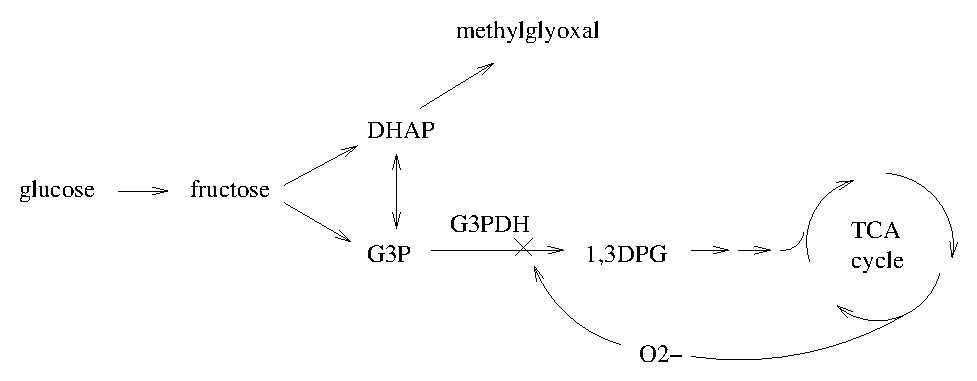
\includegraphics[width=0.75\textwidth]{figures/glycolysis} 
    \end{center}
    in order to estimate rate parameters, predict responses to
    changes, and understand the system.
}

\subsection{Components}
\frame{
  \frametitle{Combine 3 components:}
    \begin{enumerate}
     \item \emph{Biochemistry} - Biochemical components \& relationships 
     \item \emph{Mathematical Model} - Structure of relationships between components
     \item \emph{Statistical Model} - Relationship between previous information,
                             model and measured data \\
    \end{enumerate}

%  \begin{block}{Method:}
%    \begin{center}
%    ``Wrap'' standard deterministic mathematical model describing a
%    biochemical pathway within a Bayesian statistical model 
%    \end{center}
%  \end{block}

}  

\section{Aside 1: Bayesian Statistics}
\subsection{Concepts}
\frame{
  \frametitle{Bayesian Statistics: Concepts}
  \begin{enumerate}
  \item Strong Foundation from Decision Theory
  \item Modeling Process:
    \begin{enumerate}
    \item Construct a model for observed data: {\color{blue} ``Likelihood'':
      $L(\mathit{Data}|\theta)$ }
    \item Describe current information about model parameters:
      { \color{green} ``Prior distribution'' $\pi(\theta)$ }
    \item Run experiment \& collect data
    \item Apply Bayes Rule $\to$ {\color{red}``Posterior distribution''}

\begin{equation}\label{BayesRule}
{\color{red}\pi(\theta|\mathit{Data})} = \frac{{\color{blue}L(\mathit{Data}|\theta)} {\color{green}\pi(\theta)}}{\int {L(\mathit{Data}|\theta) \pi(\theta)}d\theta}
\end{equation}

    \item Draw conclusions using Posterior
    \end{enumerate}
  \end{enumerate}
}

\subsection{Bayes Rule in Pictures}

\newcommand{\doplot}[1]{%
\frame{%
  \frametitle{Bayesian Statistics: Bayes Rule in Pictures}
  \begin{center}%
    \includegraphics[height=0.75\textheight]{Posterior_00#1}%
  \end{center}%
}%
}

\doplot{1}
\doplot{2}
\doplot{3}
\doplot{4}
\doplot{5}
\doplot{6}
\doplot{7}


\subsection{Strengths \& Weaknesses}
\frame{
  \frametitle{Bayesian Statistics: Strengths \& Weaknesses}
  \begin{itemize}
  \item Strengths
    \begin{itemize}
    \item Very flexible
    \item Consistent with human thinking
    \item Allows inclusion of existing domain knowledge
    \end{itemize}
  \item Weaknesses
    \begin{itemize}
    \item Characterization of ``current information'' can be
      controversial
    \item Computationally expensive 
    \item Less popular than Frequentist statistics
    \end{itemize}
  \end{itemize}
}

\section{Aside 2: Data Cloning}
\subsection{Concepts}
\frame{
  \frametitle{Data Cloning: Concepts}
  \begin{enumerate}
  \item Leverages Bayesian MCMC approach \emph{to}
  \item Obtain Maximum likelihood estimates and standard errors (Frequentist)
  \item Process:
    \begin{enumerate}
    \item Construct a Bayesian model for observed data
    \item Fit $k$ \emph{replicates} of the observed data
    \item Increase $k$ until no change is observed
    \end{enumerate}
  \item Result: Bayesian posterior is asymptotically Normal with
    \begin{enumerate}
      \item $ \text{Mean} \to \text{MLE} $
      \item Variance 
        $\to \frac{1}{\sqrt{k n}} (\text{Fishers Information})^{-1} 
        = \frac{1}{\sqrt{k}} (\text{Standard Error}) $
      \end{enumerate}
  \end{enumerate}
}

\subsection{Strengths \& Weaknesses}
\frame{
  \frametitle{Data Cloning: Strengths \& Weaknesses}
  \begin{itemize}
  \item Strengths
    \begin{itemize}
    \item Very flexible
    \item Provides standard \emph{Frequentist} MLE estimates
    \item Not dependent on Bayesian Prior
    \end{itemize}
  \item Weaknesses
    \begin{itemize}
    \item Computationally expensive 
    \item Current software support is limited
    \end{itemize}
  \end{itemize}
}

\section{Evaluation Approach}

\frame{
  \frametitle{Reminder}
  \begin{block}{Goal: Model Biochemical Pathways}
    Estimate key rate parameters of biological pathways, e.g

    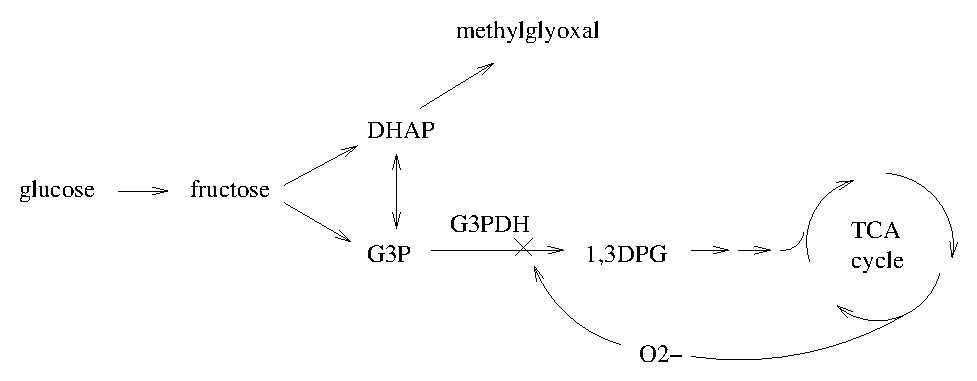
\includegraphics[width=0.75\textwidth]{figures/glycolysis} 

    in order to estimate rate parameters, predict responses to
    changes, and understand the system.
  \end{block}
}


\frame{
  \frametitle{Evaluation Approach}
  \begin{enumerate}
  \item{Create artificial model}
  \item{Generate artificial data}
  \item{Construct Mathematical + Bayesian Model}
  \item{Fit constructed model}
  \item{Compare results to known truth}
  \end{enumerate}
}

\section{Simulation Setup}
\subsection{Pathway Structure}
\frame{
  \frametitle{Pathway Structure}

  \begin{itemize}
  \item   Relationship Diagram:
    \footnotesize
    \begin{reaction} source \yields R1 \yields R2 \yields
      R3 \yields R4 \yields R5 \yields sink 
    \end{reaction}
    \normalsize
  \item
    Chemical Equations: \vspace{-5pt}
    \begin{columns}
      \footnotesize
      \begin{column}[c]{4cm}\
        \begin{chemarray*}
          source &\yields^{k_1}& R1\\
          R1 + E1 &\eqbm^{k_2}_{k_3}& R1E1 \yields^{k_4} R2 + E1\\
          R2 + E2 &\eqbm^{k_5}_{k_6}& R2E2 \yields^{k_7} R3 + E2\\
        \end{chemarray*}
      \end{column}
      \begin{column}[c]{4cm}
        \begin{chemarray*}
          R3 + E3 &\eqbm^{k_8}_{k_9}& R3E3 \yields^{k_{10}} R4 + E3\\
          R4 + E4 &\eqbm^{k_{11}}_{k_{12}}& R4E4 \yields^{k_{13}} R5 + E4\\
          R5 &\yields^{k_{14}}& sink
        \end{chemarray*}
      \end{column}
      \normalsize
    \end{columns}
  \end{itemize}
}

\subsection{Rate constants}
\frame{
  \frametitle{Rate constants}
  \begin{center}
    \begin{tabular}{c|r c c|r}
      rate constant & value & ~ & rate constant & value\\
      \cline{1-2}
      \cline{4-5}
      $k_1$ &  1.600  & ~ &  $k_8$ & 0.090 \\   
      $k_2$ &  0.540  & ~ &  $k_9$ & 4.560 \\   
      $k_3$ & 19.500  & ~ & $k_{10}$ & 1.400 \\
      $k_4$ &  2.125  & ~ & $k_{11}$ & 0.106 \\
      $k_5$ &  0.190  & ~ & $k_{12}$ & 3.670 \\
      $k_6$ &  8.460  & ~ & $k_{13}$ & 1.640 \\
      $k_7$ &  2.077  & ~ & $k_{14}$ & 0.400 \\
      \cline{1-2}
      \cline{4-5}
    \end{tabular}
  \end{center}
}

\subsection{Data Generation}
\frame{
  \frametitle{Data Generation}
  \begin{itemize}
  \item Use Gillespie's method to generate ``observed'' data
  \item Start at equilibrium
  \item Add bolus of $R1$ at time $20$.
    \vspace{-0.125in}
    \begin{center}
      \label{pulse}
      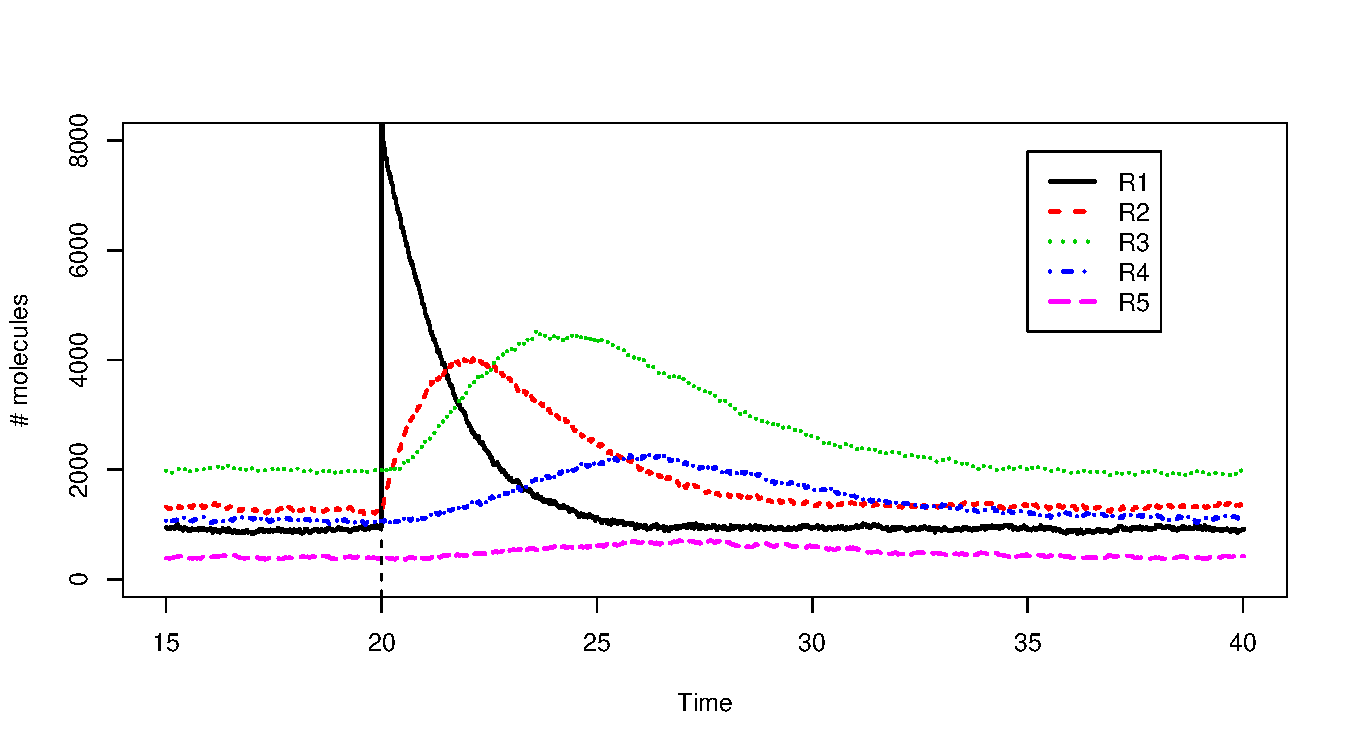
\includegraphics[height=0.5\textheight]{figures/tempDir/pulse}
    \end{center}
    \vspace{-0.125in}
  \item Triplicate estimates of reactant concentrations every minute
  \item Estimate 'velocity' via locally linear smoother, avoiding spike..
  \end{itemize}

}
 
\section{Model Specification}

\subsection{What do we need?}
\frame{
  \frametitle{Model Specification: What do we need?}
  \begin{itemize}
  \item Relationship between parameters and observable data: \vspace{-10pt}
    \begin{itemize}
    \item Biochemical model
    \item Error structure
    \end{itemize}
  \item Priors for parameters
  \item Observed Data
  \item Fitting Method
  \end{itemize}
}
 
\subsection{Biochemical Models}
\frame{
  \frametitle{Michaelis-Menten}
  
  Individual reactions were fit using the Michaelis-Menten equation
  for individual enzymes. This is a reaction of the form
  \begin{reaction}\label{eqnForm}
    E + S \eqbm^{k_1}_{k_2} ES \yields^{k_3} E + P
  \end{reaction}
  where
  \begin{eqnarray*}
    S &=& \text{substrate concentration}\\
    E &=& \text{free enzyme concentration}\\
    ES &=& \text{concentration of the enzyme-substrate complex}\\
    P &=& \text{product concentration}
  \end{eqnarray*}
}

\frame{
  \frametitle{Steady State}
    In a steady state the rate
    of the reaction $v$ is
    \begin{equation}
    v = \frac{V_{max}S}{K_m+S} 
    \end{equation}
    where
    \begin{eqnarray*}
      V_{max} &=& (E+ES)k_3 = \text{maximum reaction velocity}\\[2mm]
      K_m &=& \frac{k_2+k_3}{k_1} = \text{substrate concentration at
      half-maximal velocity}
    \end{eqnarray*}
    This form of the equation is very useful because $v$ and $S$ are
    usually measurable and $V_{max}$ and $K_m$ can be obtained by
    fitting  equation 3 to the data. I

    %In contrast, modeling $v$ as a
%    function of the individual rate constants is less useful because
%    that requires the measurement of the concentration of the
%    enzyme-substrate complex which is technically difficult.
}

\frame{
  \frametitle{Non-steady state}
    In this application we are dealing with sequences of reactions
    which are not in a steady state, so we cannot use the
    Michaelis-Menten equation directly. Instead, we use equations
    of the form
    \begin{equation}
    v = \frac{aS}{b+S} - \frac{cP}{d+P} 
  \end{equation}
    
  The coefficients $a$, $b$, $c$, and $d$ in the equations can be
  estimated with data obtained following a change in the
  concentration of one of the reactants. For example, for the data
  plotted in Slide~\ref{pulse}:
    \begin{align*}
      \deriv{R2}{t} &= v_2 = \frac{d_1R1}{d_2 + R1} -
      \frac{d_3R2}{d_4 + R2}\\[5mm]
    \end{align*}
}


\subsection{Error distribution}

\frame{
  \frametitle{Error distribution}
  The error in the velocity estimates is assumed
  to be $N(0,\sigma^2)$ so that the reaction velocities $v_j$ have a
  normal distribution:
  \[
  v_j \sim N(\mu_j,\sigma^2)
  \]

  where
  \[
  \mu_j = \frac{aS_j}{b+S_j} - \frac{cP_j}{d+P_j} 
  \]
}

\frame{
  \frametitle{Likelihoods}
  Putting this together yields:
  \footnotesize
  \begin{align*}
    v_2 &\sim N\left(\frac{d_1R1}{d_2+R1} -
      \frac{d_3R2}{d_4+R2}, \;\; \sigma^2\right)\\
    v_3 &\sim N\left(\frac{d_3R2}{d_4+R2} -
      \frac{d_5R3}{d_6+R3}, \;\; \sigma^2\right)\\
    v_4 &\sim N\left(\frac{d_5R3}{d_6+R3} -
      \frac{d_7R4}{d_8+R4}, \;\; \sigma^2\right)\\
    \intertext{\normalsize and}
    v_5 &\sim N\left(\frac{d_7R4}{d_8+R4} - d_9R5, \;\; \sigma^2\right)
  \end{align*}
}

\subsection{Prior Distributions}

\frame{
  \frametitle{Prior Distributions}

  For coefficients $d_1$ -- $d_5$: 
  \[
  \frac{3d_i}{\mu_i} \sim \chi_5^2
  \]
  where $\mu_i$ is a prior estimate of the parameter values.
  
  ~ 

  For $\sigma^2$:
  \[
  \sigma \equiv 2
  \]
  }

\section{Fitting}

\subsection{Algorithms}
\frame{
  \frametitle{Fitting algorithms}
  
  We applied 3 different MCMC algorithms (in order of shortest to
  longest required run length) as implemented in the \textsc{Hydra}
  MCMC library for \textsc{Java}.

  \begin{enumerate}
    \item Normal Kernel Coupler
    \item Multivariate normal increment Metropolis
    \item Univariate normal increment Metropolis
  \end{enumerate}
  
  Convergence and required run-length was estimated using
  \textsc{mcgibbsit}, using $q=0.025$, $r=0.0125$, and $s=0.95$,
  which ensure reliable confidence intervals. 
}

\subsection{Aside 3: What is Markov Chain Monte Carlo?}
\frame{
\begin{block}{What is Markov Chain Monte Carlo?}

\textcolor{blue}{Markov Chain Monte Carlo (MCMC)} is a technique for
generating \textcolor{red}{dependent} samples (a Markov Chain) from a
distribution without needing the \textcolor{blue}{normalizing constant}.

\end{block}
\begin{block}{When is MCMC useful?}

\textcolor{blue}{MCMC} is useful when it is \textcolor{red}{difficult} to
\textcolor{blue}{simulate} from the target distribution, such as when the
\textcolor{blue}{normalizing constant} is difficult or impossible to
compute and \textcolor{blue}{rejection sampling} is not possible.

Examples:
\begin{itemize}
  \item Sampling from \textcolor{blue}{Bayesian Posterior Distributions}
  \item Computing \textcolor{blue}{Maximum-Likelihood tests for intractable
    likelihoods}
\end{itemize}

\end{block}

}

\frame{
\frametitle{MCMC In pictures}
\begin{center}
\includegraphics[height=0.75\textheight]{MCMC-Picture}
\hfill
\includegraphics[height=0.75\textheight]{MCMC-Histogram}
\hfill
\hfill
\end{center}
}

\subsection{Algorithm Performance}
\frame{
  \frametitle{Algorithm Performance}
  \begin{center}
    \small
    Mean Squared Residuals \\
    ~

    \begin{tabular}{c||c|c|c||c|c|c}
       &
       \multicolumn{3}{c||}{mean residual SSQ $\times 10^{-4}$} & \multicolumn{3}{c}{$R_{adj}^2$}\\
      \cline{2-7}
      algorithm & 12 pt. & 16 pt. & 25 pt. &
      12 pt. & 16 pt. & 25 pt.\\
      \hline
       1-comp & 1.34 & 0.83 & 1.06 & 0.87 & 0.92 & 0.86\\
       all-comp & 0.74 & 0.93 & 0.74 & 0.93 & 0.90 & 0.90 \\
       NKC & 0.86 & 0.73 & 0.71 & 0.92 & 0.92 & 0.91
    \end{tabular}
  \end{center}
}

\frame{
  \frametitle{Fit Quality  vs. Iteration}
  \begin{center}
    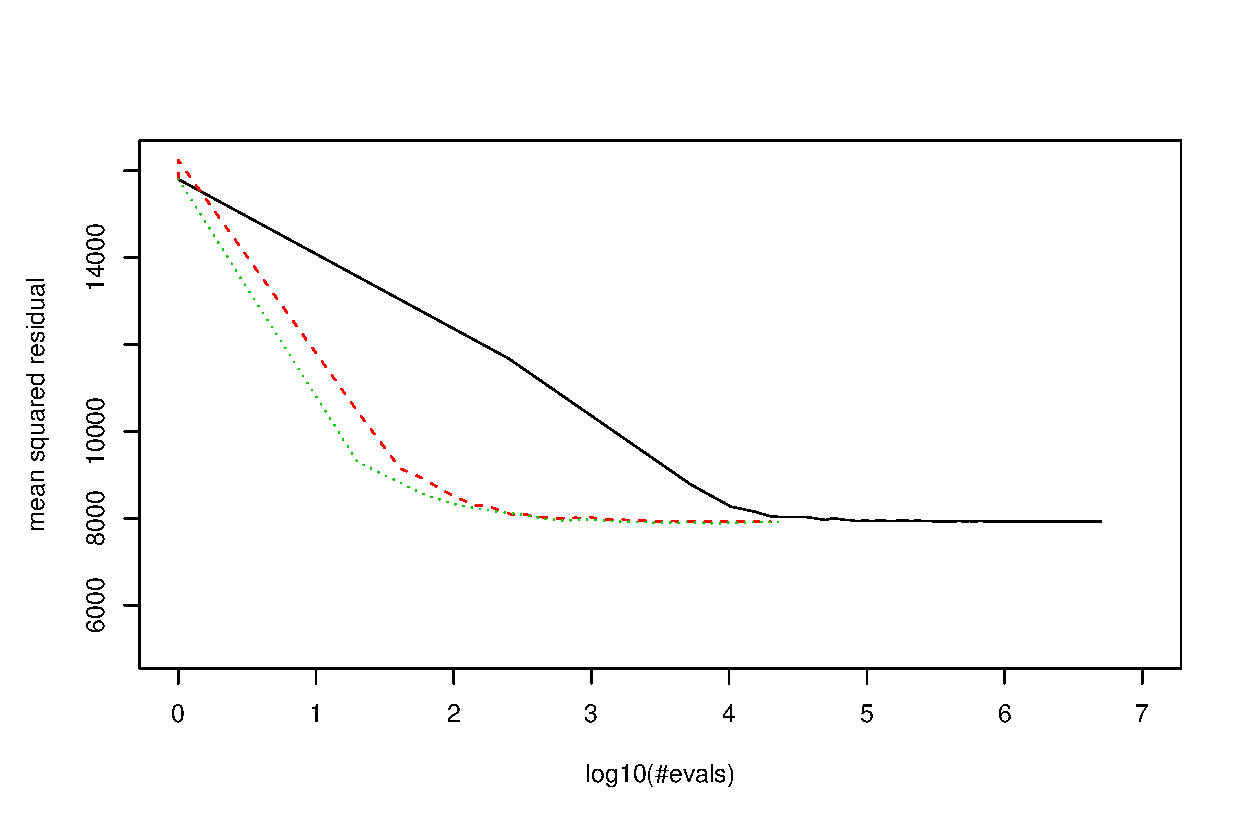
\includegraphics[width=\textwidth]{figures/MSR16}
  \end{center}
}


\section{Results}

\subsection{Posterior Distributions}
\frame{
  \frametitle{Posterior Distributions}
  
  
  \begin{columns}[c]
  \column{2in} 

  Bivariate scatter plots of the parameter distributions (upper
  triangle) and correlation coefficients (lower triangle). 

  ~

  Note the strong correlation between some pairs of parameters,
  e.g., $d_1$ -- $d_2$.

  \column{2in}

  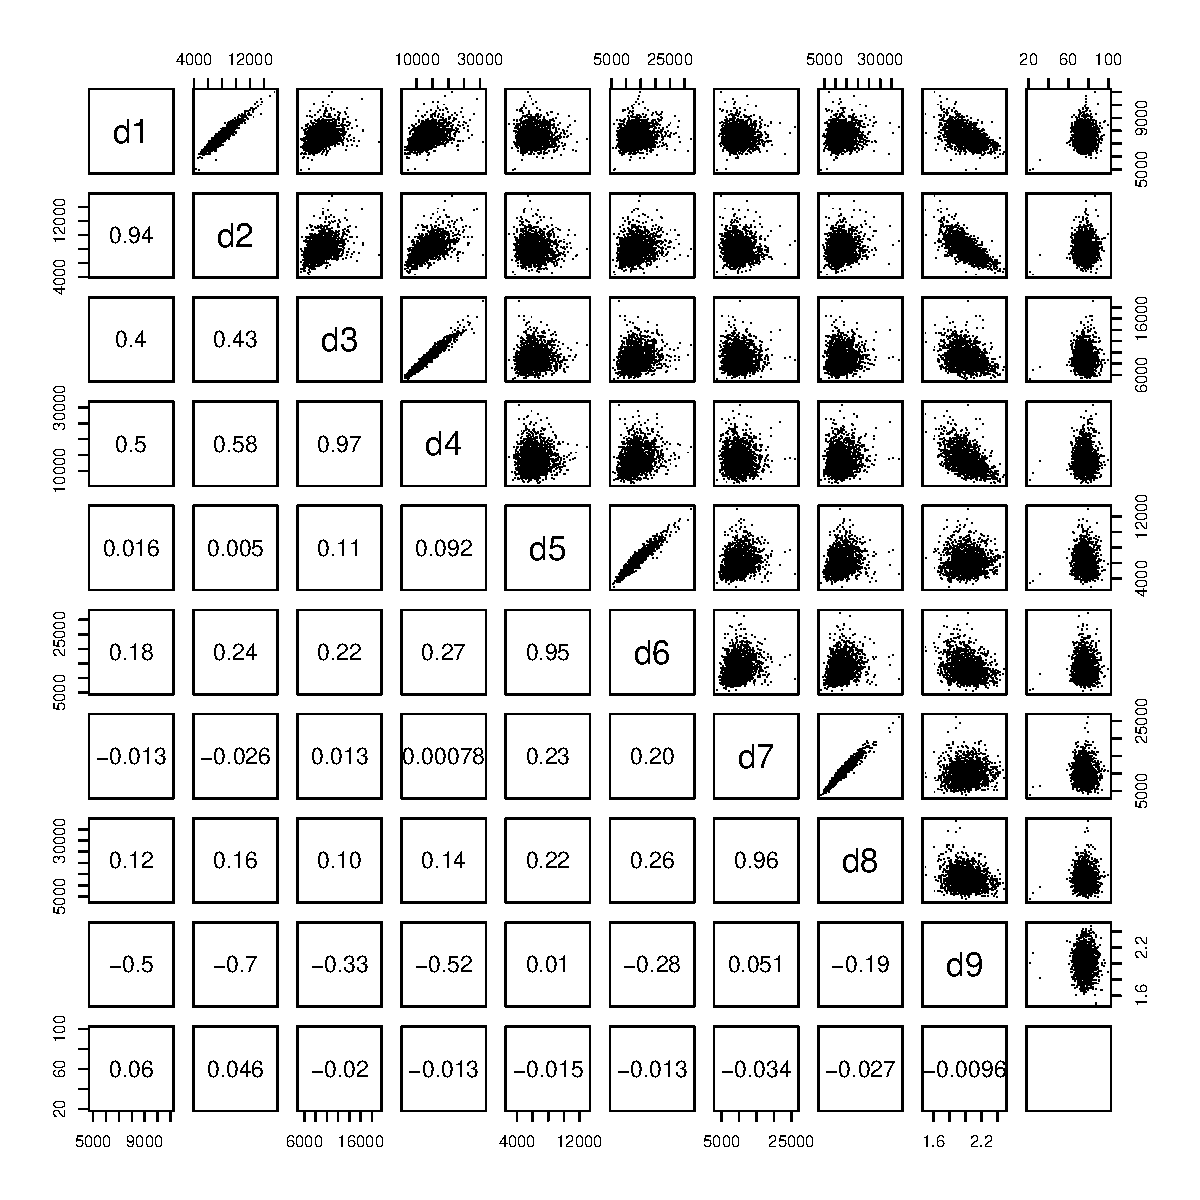
\includegraphics[width=2in]{figures/tempDir/scatterPlot}
  \end{columns}
}

\subsection{Observed vs. Fitted Values}
\frame{
  \frametitle{Observed vs. Fitted Values}

  \begin{center}
  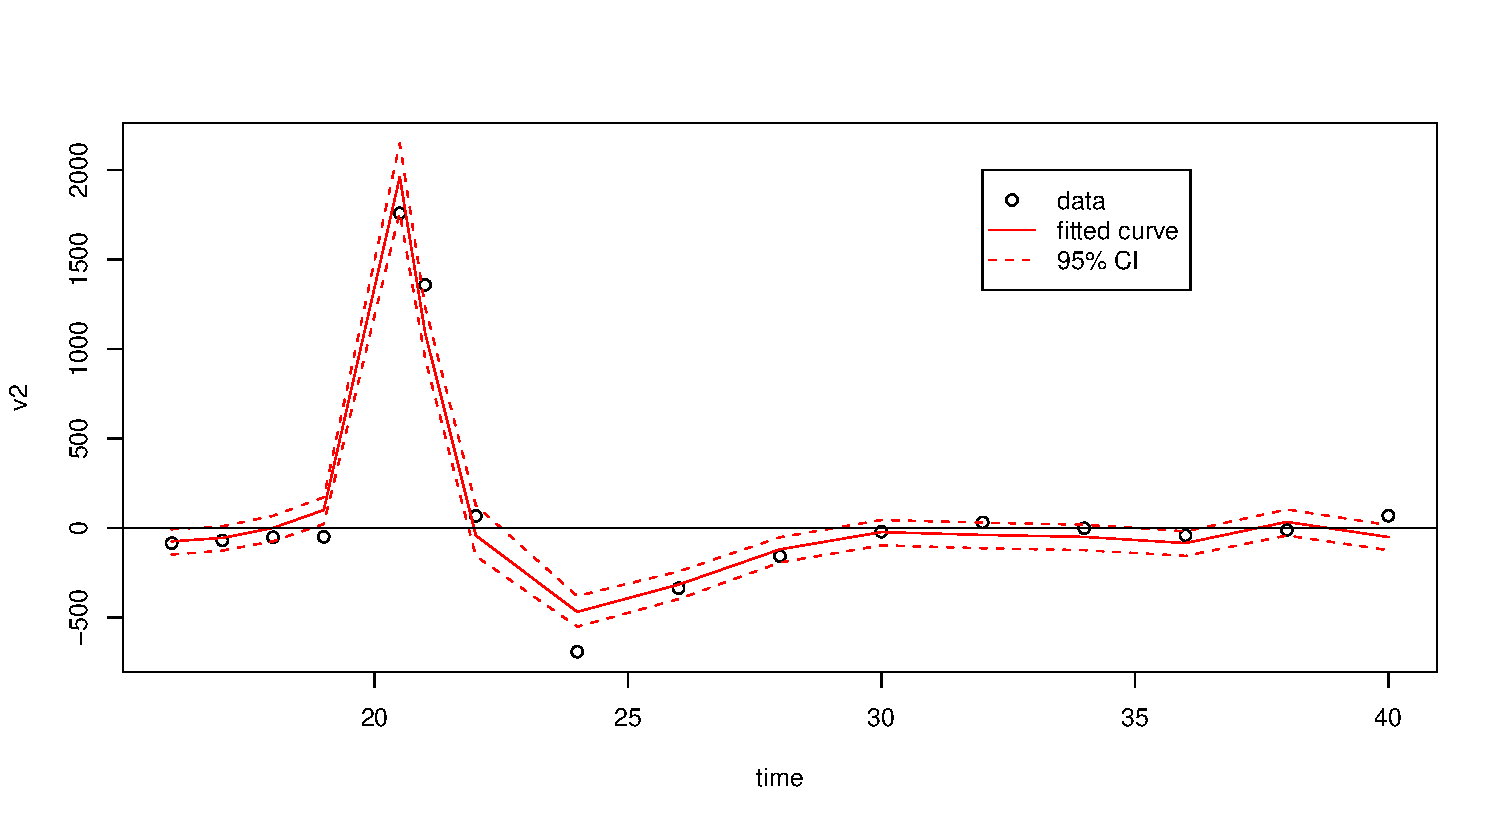
\includegraphics[width=0.5\textwidth]{figures/tempDir/V1fitted}
  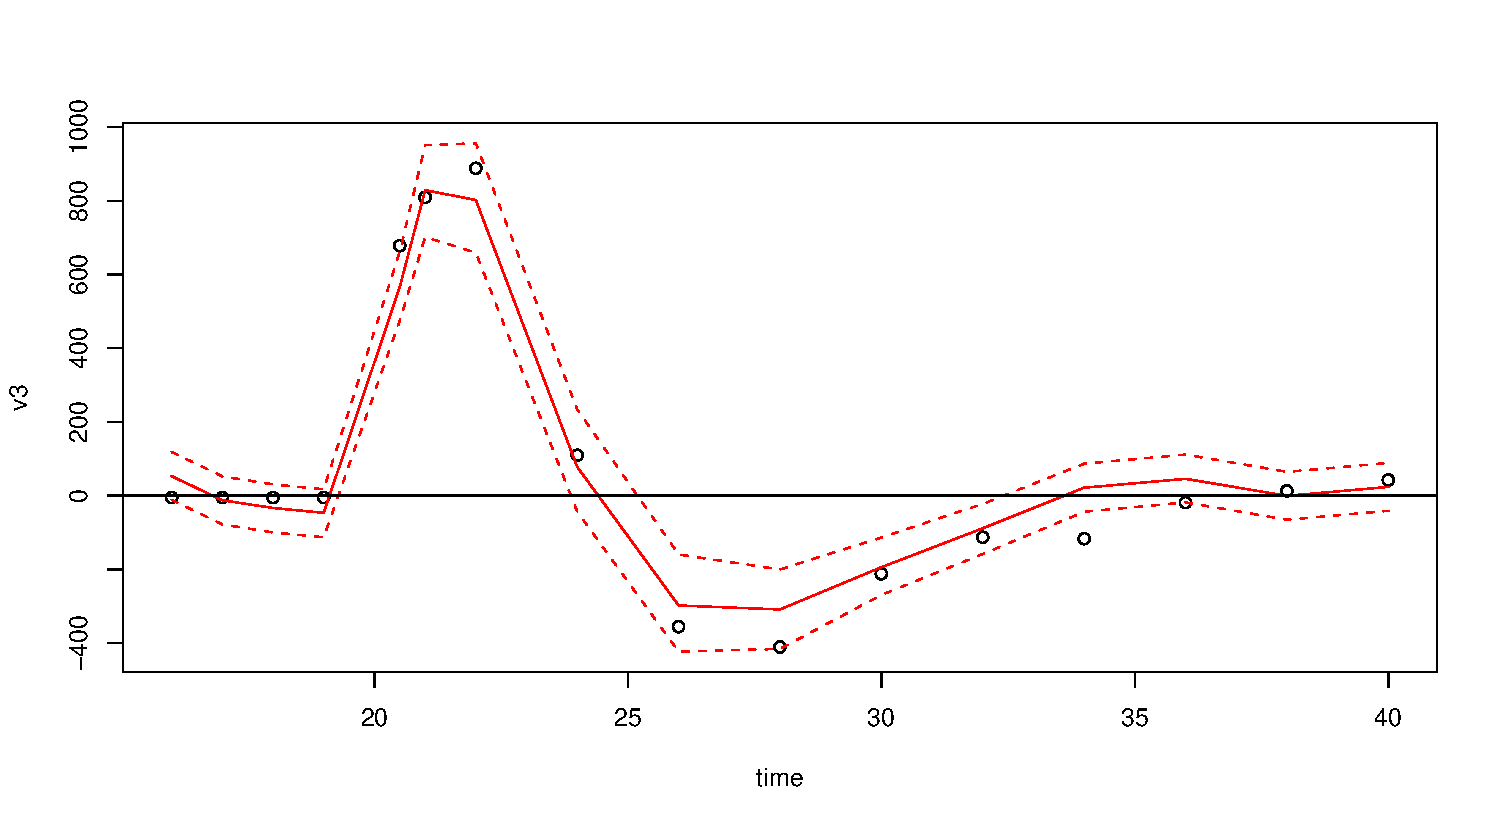
\includegraphics[width=0.5\textwidth]{figures/tempDir/V2fitted} \\

  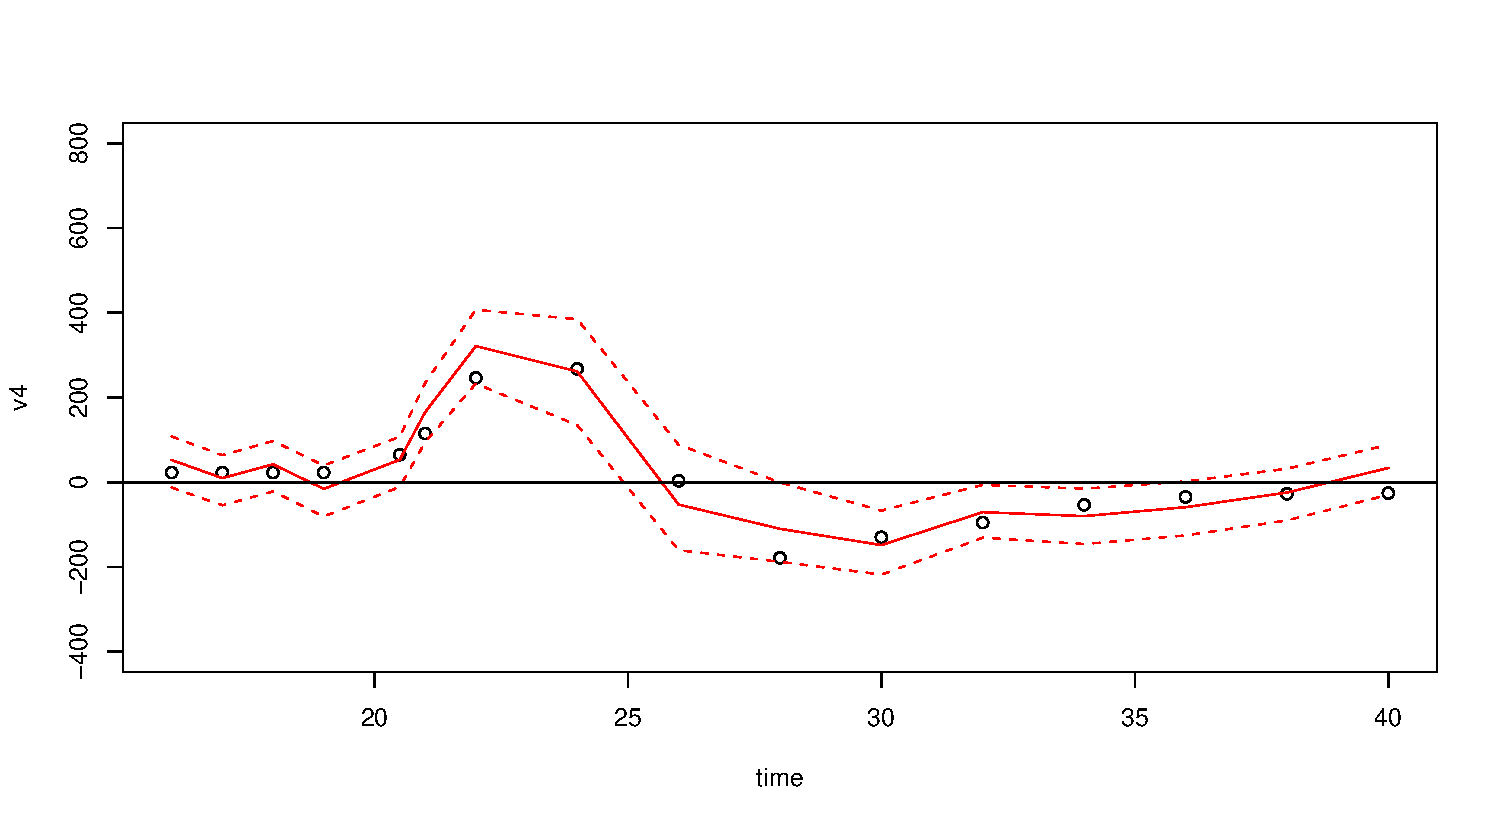
\includegraphics[width=0.5\textwidth]{figures/tempDir/V3fitted}
  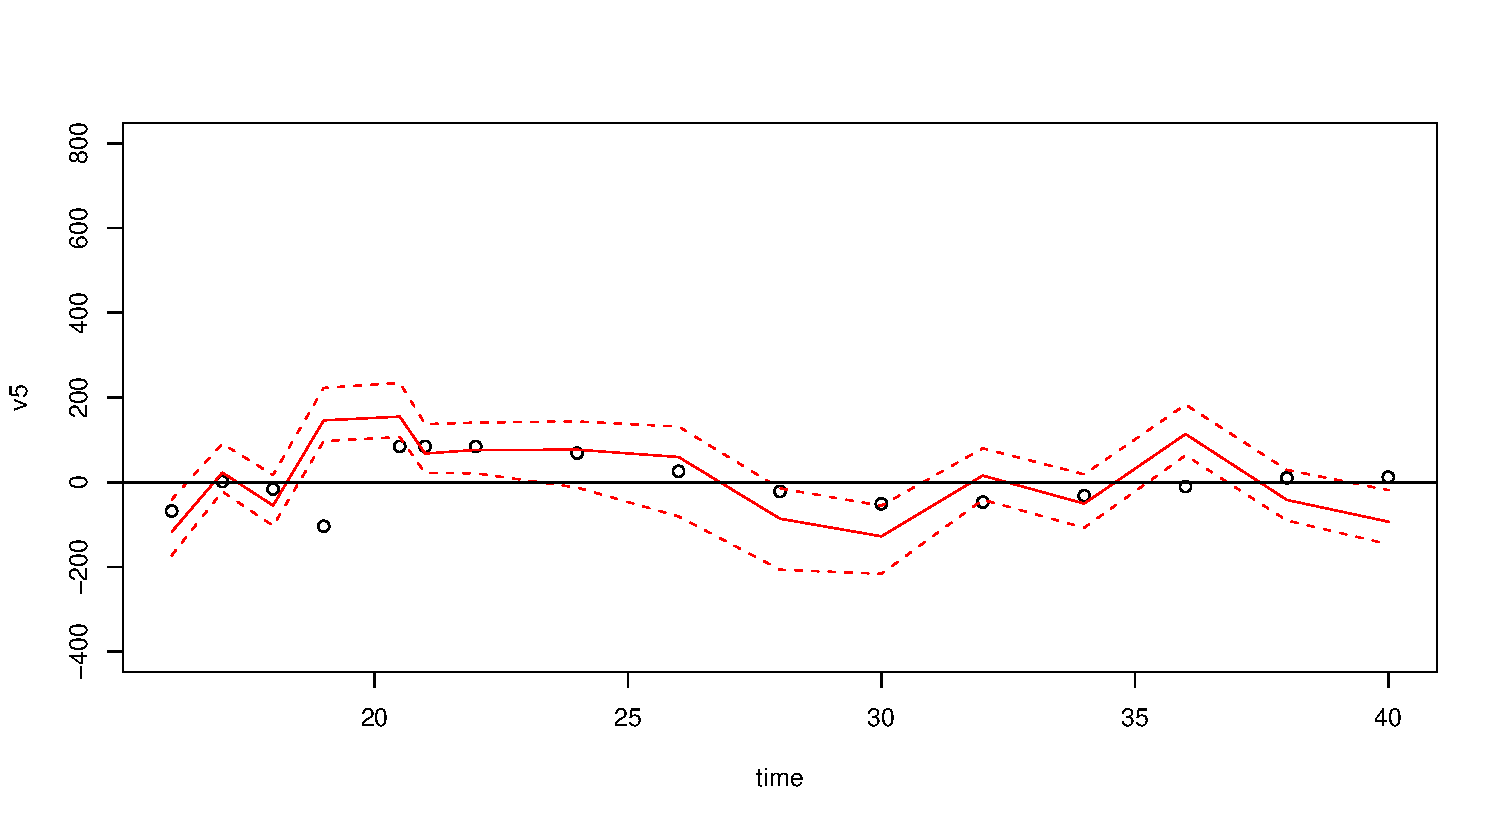
\includegraphics[width=0.5\textwidth]{figures/tempDir/V4fitted} \\
  \end{center}
}

\section{Software}

\frame{
  \frametitle{Software: DEDiscover}

  \begin{columns}
    \begin{column}[c]{0.35\textwidth}
      
\includegraphics[width=\textwidth]{Logo2.png}
    \end{column}
    \begin{column}[c]{0.65\textwidth}
      workflow-based differential equation modeling software for
      scientists, statisticians and modellers.
    \end{column}
  \end{columns}
  \begin{center}
    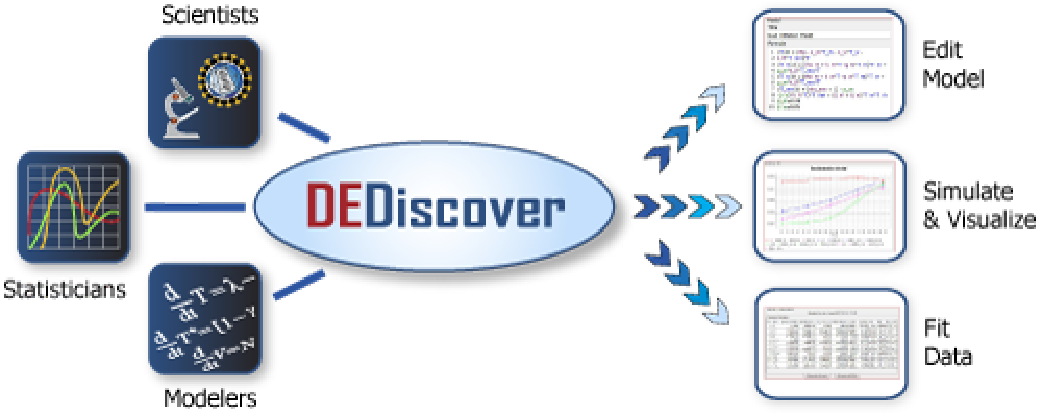
\includegraphics[width=0.8\textwidth]{DEDflow3.pdf}

    \vspace{10pt}
    \small
    \url{https://cbim.urmc.rochester.edu/software/dediscover}
  \end{center}
  
}


\section{Acknowledgments}
\frame{
  \frametitle{Acknowledgments}

  Robert "Bing" Burrows, Ph.D., who was primarily responsible for work
  described here passed away unexpectedly on December 27, 2006.

\begin{quote}
  \tiny BURROWS, ROBERT BERNARD, II, 63, of North Scituate [Rhode
  Island], died Wednesday, December 27, 2006. He was a long time
  resident of Lexington, MA before moving to Rhode Island in 2001.
  After graduating from Lexington High School, Dr. Burrows earned his
  Bachelor of Arts from Northeastern University, a Ph.D. in
  Biochemistry from the Massachusetts Institute of Technology, and a
  Master of Science in Statistics from the University of Rhode Island.
  He was a self-employed Research Biochemist and previously worked for
  the Boston Biomedical Research Institute. He leaves his sister Ellen
  Conner and her husband Donald of Coventry, his dearest friend Sally
  Glanz of North Scituate and many cousins. (\emph{The Providence
    Journal/Evening Bulletin} 2006 Dec. 31; Sec. B5)
\end{quote}
}

\section{More Information}
\frame{
  \frametitle{More Information}
  \begin{block}{Manuscript}
    \footnotesize
    Burrows~RB, Warnes~GR, Hanumara~RC, ``Statistical Modeling of Biochemical Pathways'',
    \emph{IET Systems Biology}, IET Syst. Biol. 1, 353 (2007)
  \end{block}
  \begin{block}{Contact Information}
    \footnotesize
    \begin{itemize}
    \item Email:              \url{greg@warnes.net}
%    \item Personal Web Page:  \url{http://www.warnes.net}
    \item CRC Web Page:       \url{https://www.crc.rochester.edu}
    \item CBIM Web Page:      \url{https://cbim.urmc.rochester.edu}
    \item DEDiscover:         \url{https://cbim.urmc.rochester.edu/software/dediscover}
    \item UR Biostat Web Page \url{http://www.urmc.rochester.edu/smd/biostat}
    \end{itemize}
  \end{block}
}

%%\bibliography{./refs}
%\begin{thebibliography}{99}
%  \bibitem{Oates02}%1
%    Oates,~P.J., 2002, Polyol pathway and diabetic peripheral
%    neuropathy, \emph{Int. Rev. Neurobiol.},
%    \textbf{50}, 325--392.
%  \bibitem{Gilks95} %5
%    Gilkes,~W.R., Richardson,~S., and Spiegelhalter,~D.J. (Ed.),
%    \emph{Markov Chain Monte Carlo in Practice} (Boca Raton, FL:
%    Chapman \& Hall/CRC)
%  \bibitem{R}%9
%    R Development Team, \emph{R: A Language and Environment for
%    Statistical Computing}, http://www.r-project.org (accessed 7 Nov 06)
%  \bibitem{Michaelis13} %10
%    Michaelis, L. and Menten, M.L., 1913, Die kinetic der
%    invertinwirkung, \emph{Biochem. Zeit.}, \textbf{49},
%    333--369.
%  \bibitem{Hydra}%13
%    Warnes, G.R., Hydra {MCMC} {L}ibrary,
%    http://www.sourceforge.net/projects/hydra-mcmc 
%  \bibitem{Warnes00} %14
%    Warnes, G.R., 2000, The {N}ormal {K}ernel {C}oupler: {A}n adaptive
%    {M}arkov chain {M}onte {C}arlo method for efficiently sampling
%    from multi-modal distributions, thesis, University of Washington.
%  \bibitem{projo}%16
%    OBITUARIES-SCITUATE-BURROWS. \emph{The Providence Journal/Evening
%      Bulletin} 2006 Dec. 31; Sec. B5
%  \bibitem{Lele-1}%17
%    S.R. Lele, B. Dennis, and F. Lutscher, Data Cloning: easy
%    maximum likelihood estimation for complex ecological models
%    using Bayesian Markov chain Monte Carlo methods. \emph{Ecology
%      Letters}, 10:551-563, 2007.
%  \bibitem{Lele-2}%18
%    S.R. Lele, K. Nadeem, and B. Schuland. Estimability and likelihood
%    inference for generalized linear mixed models using data cloning.
%    \emph{Jornal of the Americal Statistical Association} 2010. in
%    press.
%  \bibitem{Ponciano}%19
%    J.M. Ponciano, M.L. Taper, B. Dennis, and S.R. Lele. Hierarchical
%    models in ecology: confidence intervals, hypothesis testing, and
%    model selection using data cloning. \emph{Ecology}, 90:356-362,
%    2009.
%\end{thebibliography}




\end{document}
